\documentclass[]{article}

\usepackage[left=2.00cm, right=2.00cm, top=2.00cm, bottom=2.00cm]{geometry}
\usepackage[spanish,es-noshorthands]{babel}
\usepackage[utf8]{inputenc} % para tildes y ñ
\usepackage{graphicx} % para las figuras
\usepackage{xcolor}
\usepackage{listings} % para el código fuente en c++

\lstdefinestyle{customc}{
  belowcaptionskip=1\baselineskip,
  breaklines=true,
  frame=single,
  xleftmargin=\parindent,
  language=C++,
  showstringspaces=false,
  basicstyle=\footnotesize\ttfamily,
  keywordstyle=\bfseries\color{green!40!black},
  commentstyle=\itshape\color{gray!40!gray},
  identifierstyle=\color{black},
  stringstyle=\color{orange},
}
\lstset{style=customc}


%opening
\title{Práctica 1. Algoritmos devoradores}
\author{Juan Carlos Lucena Monje \\ % mantenga las dos barras al final de la línea y este comentario
juancarlos.lucenamonje@alum.uca.es \\ % mantenga las dos barras al final de la línea y este comentario
Teléfono: 637929532 \\ % mantenga las dos barras al final de la linea y este comentario
NIF: 45899713q \\ % mantenga las dos barras al final de la línea y este comentario
}


\begin{document}

\maketitle

%\begin{abstract}
%\end{abstract}

% Ejemplo de ecuación a trozos
%
%$f(i,j)=\left\{ 
%  \begin{array}{lcr}
%      i + j & si & i < j \\ % caso 1
%      i + 7 & si & i = 1 \\ % caso 2
%      2 & si & i \geq j     % caso 3
%  \end{array}
%\right.$

\begin{enumerate}
\item Describa a continuación la función diseñada para otorgar un determinado valor a cada una de las celdas del terreno de batalla para el caso del centro de extracción de minerales. 

Calculo el valor en funcion de la distancia a la que este de los obstaculos. Utilizo un incrementador para clasificar las distancias, consiguiendo que a mayor distancia haya menos valor tendra.

% Elimine los símbolos de tanto por ciento para descomentar las siguientes instrucciones e incluir una imagen en su respuesta. La mejor ubicación de la imagen será determinada por el compilador de Latex. No tiene por qué situarse a continuación en el fichero en formato pdf resultante.
\begin{figure}
\centering
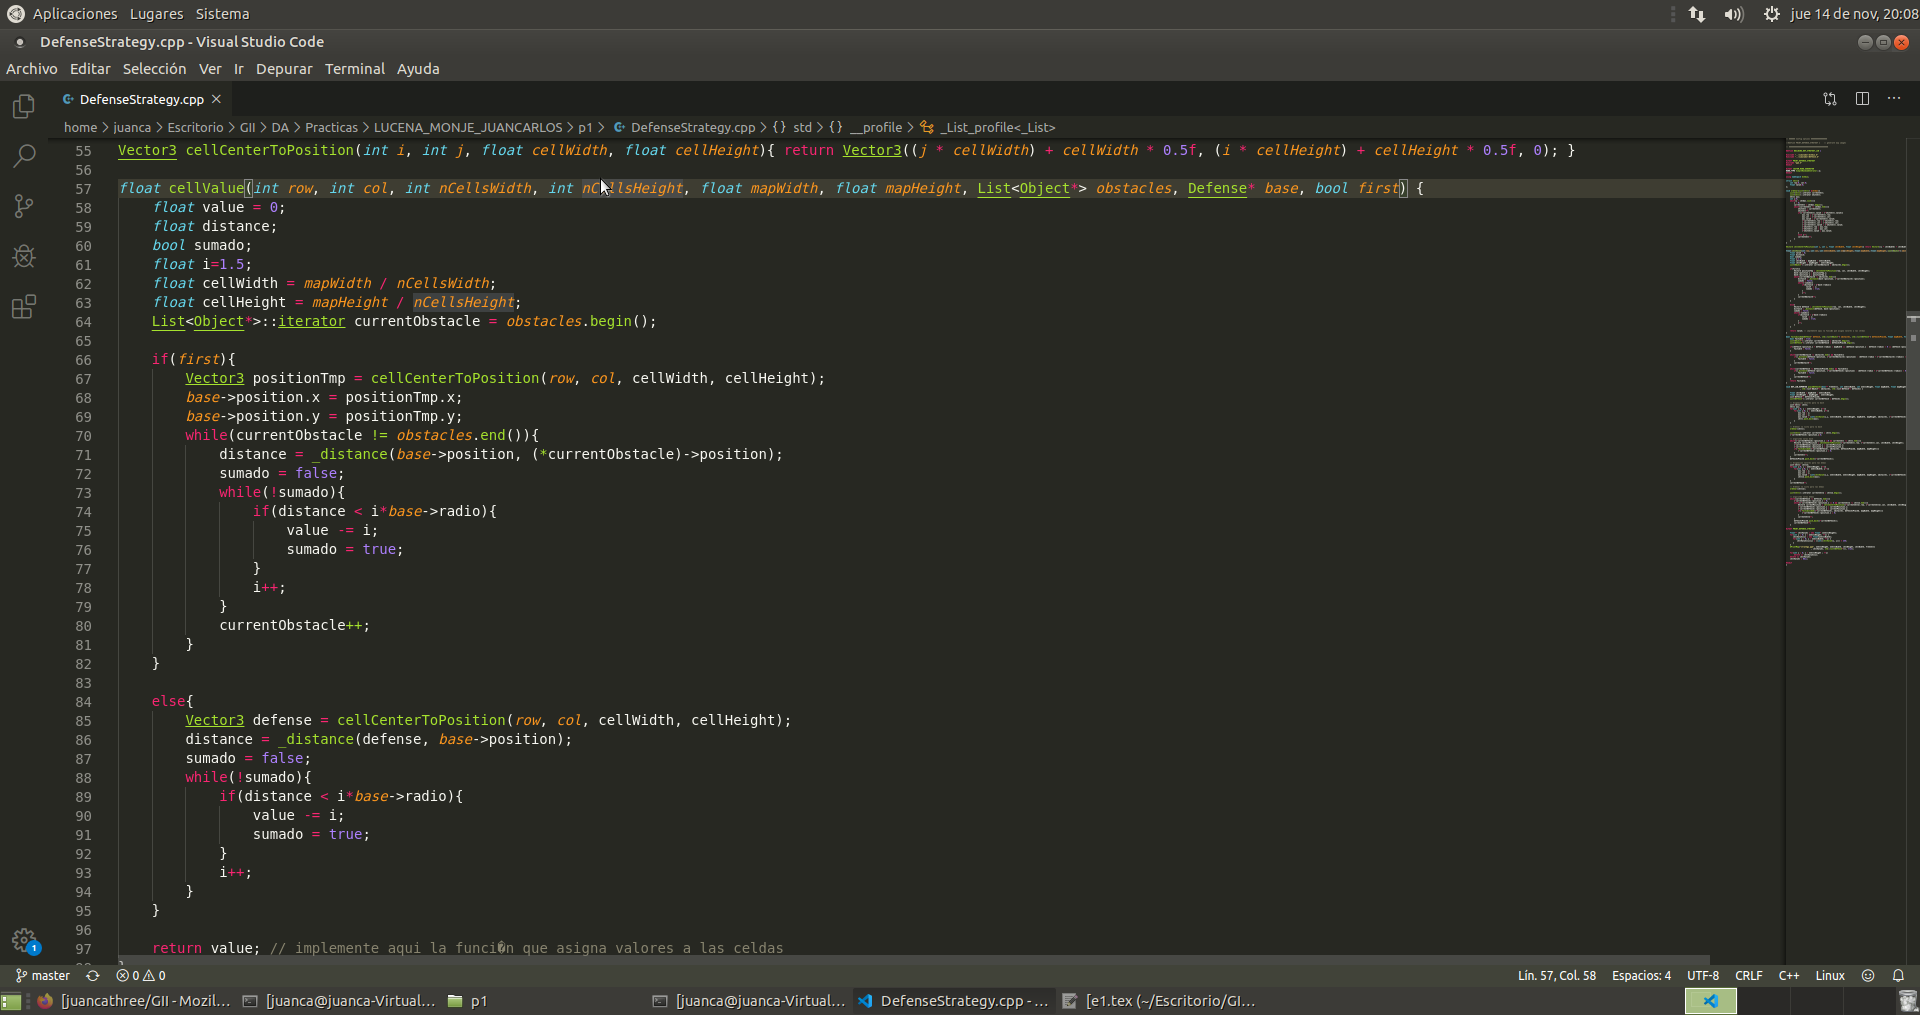
\includegraphics[width=0.7\linewidth]{./defenseValueCellsHead} % no es necesario especificar la extensión del archivo que contiene la imagen
\caption{Estrategia devoradora para la mina}
\label{fig:defenseValueCellsHead}
\end{figure}


\item Diseñe una función de factibilidad explicita y descríbala a continuación.

Escriba aquí su respuesta al ejercicio 2.

\item A partir de las funciones definidas en los ejercicios anteriores diseñe un algoritmo voraz que resuelva el problema para el caso del centro de extracción de minerales. Incluya a continuación el código fuente relevante. 

Escriba aquí su respuesta al ejercicio 3.

\item Comente las características que lo identifican como perteneciente al esquema de los algoritmos voraces. 

Una vez haya seleccionado una celda del conjunto si es valida se asigna y ya no puede excluirse y en el caso de que no sea valida no se vuevlve a tener nunca en cuenta.


\item Describa a continuación la función diseñada para otorgar un determinado valor a cada una de las celdas del terreno de batalla para el caso del resto de defensas. Suponga que el valor otorgado a una celda no puede verse afectado por la colocación de una de estas defensas en el campo de batalla. Dicho de otra forma, no es posible modificar el valor otorgado a una celda una vez que se haya colocado una de estas defensas. Evidentemente, el valor de una celda sí que puede verse afectado por la ubicación del centro de extracción de minerales.

Escriba aquí su respuesta al ejercicio 5.

\item A partir de las funciones definidas en los ejercicios anteriores diseñe un algoritmo voraz que resuelva el problema global. Este algoritmo puede estar formado por uno o dos algoritmos voraces independientes, ejecutados uno a continuación del otro. Incluya a continuación el código fuente relevante que no haya incluido ya como respuesta al ejercicio 3. 

Escriba aquí su respuesta al ejercicio 6.

\end{enumerate}

Todo el material incluido en esta memoria y en los ficheros asociados es de mi autoría o ha sido facilitado por los profesores de la asignatura. Haciendo entrega de este documento confirmo que he leído la normativa de la asignatura, incluido el punto que respecta al uso de material no original.

\end{document}
